\pdfminorversion=4
\documentclass[10pt]{beamer}\usepackage[]{graphicx}\usepackage[]{color}
%% maxwidth is the original width if it is less than linewidth
%% otherwise use linewidth (to make sure the graphics do not exceed the margin)
\makeatletter
\def\maxwidth{ %
  \ifdim\Gin@nat@width>\linewidth
    \linewidth
  \else
    \Gin@nat@width
  \fi
}
\makeatother

\definecolor{fgcolor}{rgb}{0.345, 0.345, 0.345}
\newcommand{\hlnum}[1]{\textcolor[rgb]{0.686,0.059,0.569}{#1}}%
\newcommand{\hlstr}[1]{\textcolor[rgb]{0.192,0.494,0.8}{#1}}%
\newcommand{\hlcom}[1]{\textcolor[rgb]{0.678,0.584,0.686}{\textit{#1}}}%
\newcommand{\hlopt}[1]{\textcolor[rgb]{0,0,0}{#1}}%
\newcommand{\hlstd}[1]{\textcolor[rgb]{0.345,0.345,0.345}{#1}}%
\newcommand{\hlkwa}[1]{\textcolor[rgb]{0.161,0.373,0.58}{\textbf{#1}}}%
\newcommand{\hlkwb}[1]{\textcolor[rgb]{0.69,0.353,0.396}{#1}}%
\newcommand{\hlkwc}[1]{\textcolor[rgb]{0.333,0.667,0.333}{#1}}%
\newcommand{\hlkwd}[1]{\textcolor[rgb]{0.737,0.353,0.396}{\textbf{#1}}}%

\usepackage{framed}
\makeatletter
\newenvironment{kframe}{%
 \def\at@end@of@kframe{}%
 \ifinner\ifhmode%
  \def\at@end@of@kframe{\end{minipage}}%
  \begin{minipage}{\columnwidth}%
 \fi\fi%
 \def\FrameCommand##1{\hskip\@totalleftmargin \hskip-\fboxsep
 \colorbox{shadecolor}{##1}\hskip-\fboxsep
     % There is no \\@totalrightmargin, so:
     \hskip-\linewidth \hskip-\@totalleftmargin \hskip\columnwidth}%
 \MakeFramed {\advance\hsize-\width
   \@totalleftmargin\z@ \linewidth\hsize
   \@setminipage}}%
 {\par\unskip\endMakeFramed%
 \at@end@of@kframe}
\makeatother

\definecolor{shadecolor}{rgb}{.97, .97, .97}
\definecolor{messagecolor}{rgb}{0, 0, 0}
\definecolor{warningcolor}{rgb}{1, 0, 1}
\definecolor{errorcolor}{rgb}{1, 0, 0}
\newenvironment{knitrout}{}{} % an empty environment to be redefined in TeX

\usepackage{alltt}
%% O comando acima foi necessario porque o PDF nao abria no acrobat do
%% windows, dava o erro 131. Provavelmente devido as figuras em
%% PDF. Agora ele gera um PDF versao 1.4, ao inves da versao 1.5

\usetheme[compress]{PaloAlto}
\usecolortheme{sidebartab} % crane

\usepackage[brazilian]{babel}
\usepackage[T1]{fontenc}
\usepackage[utf8]{inputenc}
\usepackage{graphicx}
\usepackage{hyperref}
\usepackage[scaled]{beramono} % truetype: Bistream Vera Sans Mono
%\usepackage{inconsolata}
\usepackage{amsmath}
\usepackage{xfrac}
\usepackage{tikz}
\usepackage{xcolor}
\usepackage{multirow}
\usepackage{multicol}
\usepackage{tikz}
\usetikzlibrary{arrows, decorations.pathmorphing, backgrounds, fit,
  positioning, calc, trees, plotmarks}

\setbeamertemplate{footline}[frame number] % mostra o numero dos slides
\setbeamertemplate{navigation symbols}{} % retira a barra de navegacao

\usepackage{xspace}
\providecommand{\eg}{\textit{e.g.}\xspace}
\providecommand{\ie}{\textit{i.e.}\xspace}
\providecommand{\R}{\textsf{R}\xspace}
\newcommand{\mb}[1]{\mathbf{#1}}
\newcommand{\bs}[1]{\boldsymbol{#1}}
\providecommand{\E}{\text{E}}
\providecommand{\Var}{\text{Var}}
\providecommand{\DP}{\text{DP}}
\providecommand{\EP}{\text{EP}}
\providecommand{\N}{\text{N}}
\theoremstyle{definition}
\newtheorem*{mydef}{Definição}
\newtheorem*{mythm}{Teorema}

\title{Estimação intervalar}
\author[]{Fernando de Pol Mayer}
\institute[UFPR]{Laboratório de Estatística e Geoinformação (LEG) \\
  Departamento de Estatística (DEST) \\
  Universidade Federal do Paraná (UFPR)}
\date{}
\logo{\includegraphics[width=1.6cm]{../img/ufpr-logo.png}}
\titlegraphic{\includegraphics[width=1cm]{../img/CC_by-nc-sa_88x31.png}\\
  \tiny
  \href{https://creativecommons.org/licenses/by-nc-sa/4.0/deed.pt_BR}{Este
    conteúdo está disponível por meio da Licença Creative Commons 4.0
    (Atribuição/NãoComercial/PartilhaIgual)}}

\AtBeginSection[]
{
  \begin{frame}
    \frametitle{Plano de aula}
    \tableofcontents[currentsection]
  \end{frame}
}

\AtBeginSubsection[]
{
  \begin{frame}
    \frametitle{Plano de aula}
    \tableofcontents[currentsection,currentsubsection]
  \end{frame}
}
\IfFileExists{upquote.sty}{\usepackage{upquote}}{}
\begin{document}





\begin{frame}
\maketitle
%\titlepage
\end{frame}

\begin{frame}{Sumário}
\tableofcontents
\end{frame}

\section{Introdução}

\begin{frame}{Estimação}
  Existem dois tipos de estimativas que podemos obter a partir de uma
  \textbf{amostra aleatória}: \\~\\
  \begin{block}{Estimativa pontual}
    Fornecem como estimativa um único valor numérico para o parâmetro de
    interesse
  \end{block}
  \begin{block}{Estimativa intervalar}
    Fornece um intervalo de valores ``plausíveis'' para o parâmetro de
    interesse
  \end{block}
\end{frame}

\begin{frame}{Estimação}
  Por serem \textbf{variáveis aleatórias}, os estimadores pontuais
  possuem uma distribuição de probabilidade (distribuições amostrais)
  \\~\\
  Com isso, podemos apresentar uma estimativa mais informativa para o
  parâmetro de interesse, que inclua uma medida de \textbf{precisão} do
  valor obtido $\rightarrow$ \textbf{estimativa intervalar} ou
  \textbf{intervalo de confiança} \\~\\
  Os \textbf{intervalos de confiança} são obtidos a partir da
  \textbf{distribuição amostral} de seus estimadores
\end{frame}

\section{Intervalos de confiança para a média: $\sigma$ conhecido}

\begin{frame}{Intervalos de confiança para a média: $\sigma$ conhecido}
  Suposições necessárias
  \begin{itemize}
  \item A amostra é uma \textbf{amostra aleatória simples}. (Todas as
    amostras de mesmo tamanho tem a mesma probabilidade de serem selecionadas)
  \item O valor do desvio-padrão populacionalm $\sigma$, é conhecido
  \item Uma ou ambas das seguintes condições são satisfeitas:
    \begin{itemize}
    \item A população é normalmente distribuída
    \item A amostra possui $n > 30$
    \end{itemize}
  \end{itemize}
\end{frame}

\begin{frame}{Intervalos de confiança para a média: $\sigma$ conhecido}
  Quando coletamos uma \textbf{amostra aleatória} e calculamos uma
  média, sabemos que o valor da média possui um desvio natural, em
  relação ao verdadeiro valor da média populacional (\textbf{erro
    amostral}), ou seja
  \begin{equation*}
    e = \bar{X} - \mu \quad \Rightarrow \quad \bar{X} = \mu + e
  \end{equation*}
  \vspace{1em}

  Sabemos que a \textbf{distribuição amostral da média} é uma
  distribuição normal, com média $\mu$ e variância
  $\sigma^2/n$,
  \begin{equation*}
    \bar{X} \sim \text{N}\left(\mu, \frac{\sigma^2}{n}\right)
  \end{equation*}
\end{frame}

\begin{frame}{Intervalos de confiança para a média: $\sigma$ conhecido}
  Usando a transformação
  \begin{equation*}
    Z = \frac{\bar{X} - \mu}{\sigma/\sqrt{n}} =
    \frac{e}{\sigma/\sqrt{n}} \, \sim \, \text{N}(0,1)
  \end{equation*}
  podemos determinar o \textbf{erro máximo provável} que
  assumimos para a média amostral que estamos calculando. \\~\\
  O \textbf{erro máximo provável} ou \textbf{margem de erro} da média é
  definido por
  \begin{equation*}
    e = z_{\alpha/2} \cdot \frac{\sigma}{\sqrt{n}}
  \end{equation*}
  onde $z_{\alpha/2}$ é chamado de \textbf{valor crítico}.
\end{frame}

\begin{frame}{Valores críticos}
  O valor crítico $z_{\alpha/2}$ é o valor de $Z$ que separa uma área de
  $\alpha/2$ da cauda da distribuição normal padrão
  \begin{figure}[h]
    \centering
    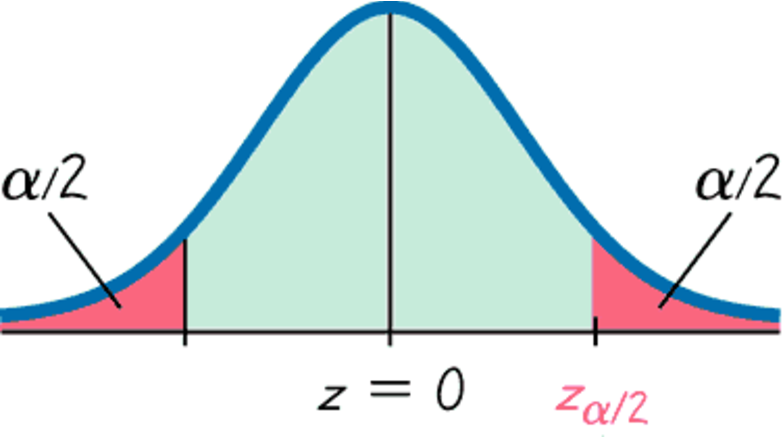
\includegraphics[width=.5\textwidth]{z_critico}
  \end{figure}
  Como estamos interessados nos valores \textbf{mais prováveis} da
  média, então nosso interesse está no centro da distribuição $Z$, que
  concentra uma área $\gamma = 1 - \alpha$, que determina o
  \textbf{nível de confiança} do intervalo
\end{frame}

\begin{frame}{Valores críticos}
  \begin{figure}[h]
    \centering
    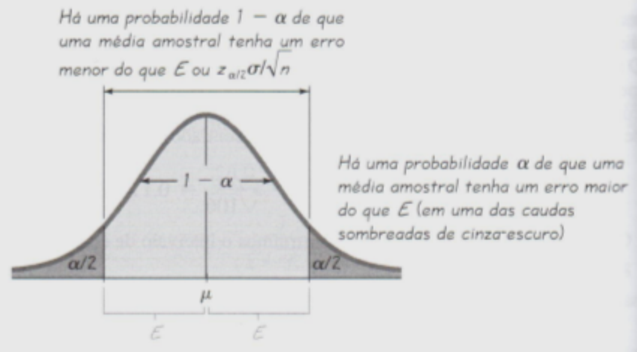
\includegraphics[width=1\textwidth]{areas}
  \end{figure}
\end{frame}

\begin{frame}{Nível de confiança}
  A área $\gamma = 1 - \alpha$ determina o \textbf{nível de confiança}
  associado ao intervalo de confiança que estamos construindo \\~\\
  O valor de $\alpha$ é o complemento do nível de confiança\\~\\
  Exemplo:
  \begin{itemize}
  \item Para um nível de confiança de 0,95 (ou 95\%), $\alpha = 0,05$
  \item Para um nível de confiança de 0,99 (ou 99\%), $\alpha = 0,01$
  \end{itemize}
  \begin{alertblock}{Importante!}
    O \textbf{nível de confiança} é a probabilidade $1-\alpha$, que é a
    proporção de vezes que o intervalo de confiança realmente contém o
    parâmetro populacional, supondo que a amostragem pudesse ser
    repetida um grande número de vezes
  \end{alertblock}
\end{frame}

\begin{frame}{Encontrando valores críticos}
  Com a definição do \textbf{nível de confiança}, sabemos então o valor
  de $\alpha$, e devemos encontrar o valor de $z_{\alpha/2}$. Usando
  como exemplo $\gamma = 0,95 = 1 - 0,05 \Rightarrow \alpha = 0,05$:
  \begin{itemize}
  \item Temos que $\alpha/2 = 0,025$ é a área em cada cauda
  \item Na tabela da distribuição normal padrão, procure a
    \textbf{área}, no corpo da tabela, que corresponde a $0,5 - 0,025 =
    0,475$
  \item O valor de $z_{\alpha/2}$ será determinado pelos valores
    correspondentes nas margens da tabela. Nesse caso, $z_{\alpha/2} =
    1,96$ é o valor crítico procurado.
  \end{itemize}
  \begin{figure}[b]
    \centering
    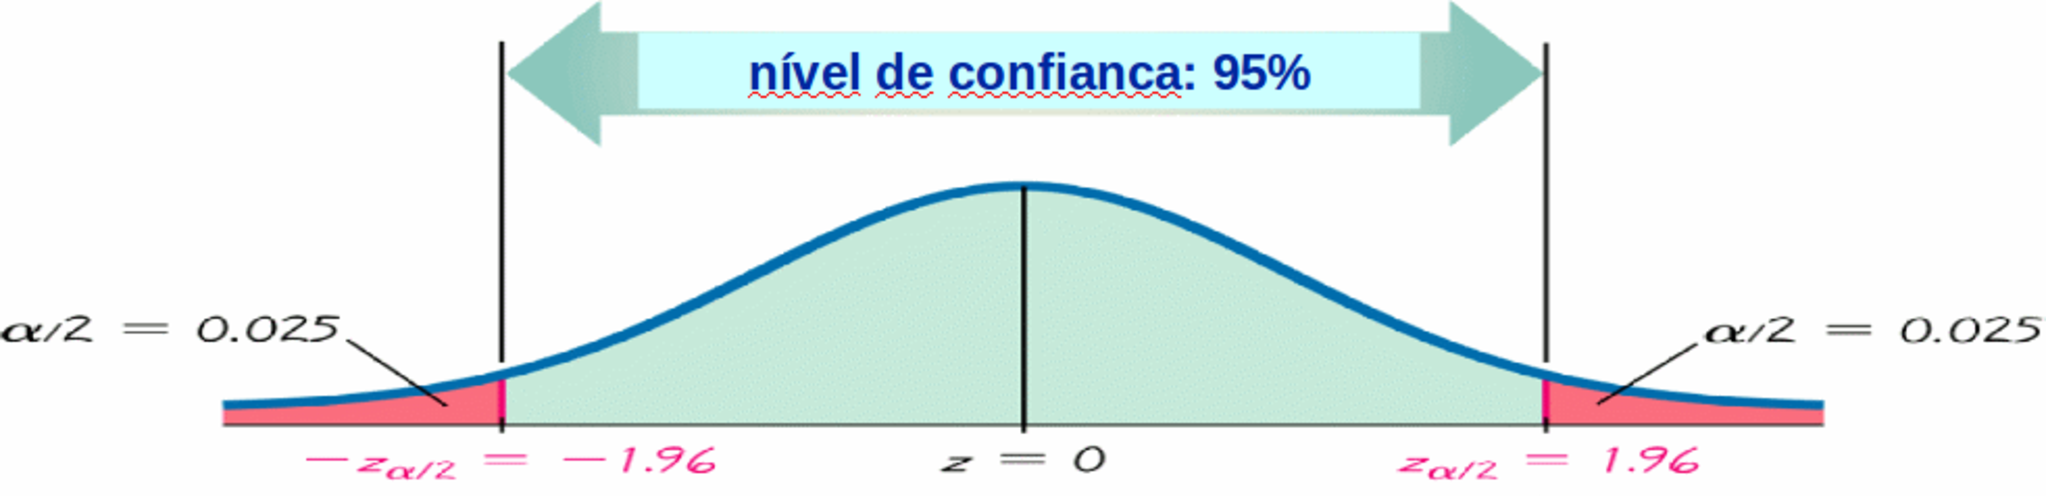
\includegraphics[width=1\textwidth]{conf}
  \end{figure}
\end{frame}

\begin{frame}{Encontrando valores críticos}
  Encontre os valores críticos para os níveis de confiança
  \begin{itemize}
  \item $\gamma = 0,90 \Rightarrow \alpha = 0,10$
  \item $\gamma = 0,99 \Rightarrow \alpha = 0,01$
  \end{itemize}
  \begin{table}[h]
    \centering
    \caption{Níveis de confiança e valores críticos mais comuns}
    \begin{tabular}{ccc}
      \hline
      Nível de confiança $\gamma$ & $\alpha$ & Valor crítico
      $z_{\alpha/2}$ \\
      \hline
      0,90 & 0,10 & 1,645 \\
      0,95 & 0,05 & 1,96 \\
      0,99 & 0,01 & 2,575 \\
      \hline
    \end{tabular}
  \end{table}
\end{frame}

\begin{frame}{Intervalos de confiança para a média: $\sigma$ conhecido}
  Com estas definições, podemos construir um \textbf{intervalo de
    confiança} para uma \textbf{estimativa amostral da média com
    $\sigma$ conhecido} através de
  \begin{equation*}
    \bar{x} - e < \mu < \bar{x} + e
  \end{equation*}
  com
  \begin{equation*}
    e = z_{\alpha/2} \cdot \left(\frac{\sigma}{\sqrt{n}}\right)
  \end{equation*}
  Outras notações
  \begin{equation*}
    \bar{x} \pm e
  \end{equation*}
  \begin{equation*}
    [\bar{x} - e; \bar{x} + e]
  \end{equation*}
\end{frame}

\begin{frame}{Intervalos de confiança para a média: $\sigma$ conhecido}
  Porque podemos fazer isso? \\~\\
  \begin{eqnarray*}
    &&\Pr[-z_{\alpha/2} < Z < z_{\alpha/2}] = \gamma \\
    &&\Pr[-z_{\alpha/2} < \frac{\bar{x} - \mu}{\sigma/\sqrt{n}} <
    z_{\alpha/2}] = \gamma
  \end{eqnarray*}
  Isolando $\mu$ nessa inequação,
  \begin{eqnarray*}
    &&\Pr[\bar{x} - z_{\alpha/2} \cdot
    \left(\frac{\sigma}{\sqrt{n}} \right) < \mu < \bar{x} + z_{\alpha/2}
    \cdot \left(\frac{\sigma}{\sqrt{n}} \right)] = \gamma \\
    &&\Pr[\bar{x} - e < \mu < \bar{x} + e] = \gamma \\
  \end{eqnarray*}
\end{frame}

\begin{frame}{Intervalos de confiança para a média: $\sigma$ conhecido}
  \textbf{Procedimentos gerais para a construção de intervalos de confiança}
  \\~\\
  \begin{enumerate}
  \item Verifique se as suposições necessárias estão satisfeitas
    \begin{itemize}
    \item Temos uma AAS
    \item $\sigma$ é conhecido
    \item A população tem distribuição normal ou $n>30$
    \end{itemize}
  \item Determine o nível de confiança $\gamma$, e identifique $\alpha$
  \item Com o valor de $\alpha$ definido, encontre o valor crítico de
    $z_{\alpha/2}$
  \item Calcule a margem de erro $e = z_{\alpha/2} \cdot (\sigma/\sqrt{n})$
  \item Coloque em um dos formatos gerais para intervalo de confiança
    \begin{itemize}
    \item[] $\bar{x} - e < \mu < \bar{x} + e$
    \item[] $\bar{x} \pm e$
    \item[] $[\bar{x} - e; \bar{x} + e]$
    \end{itemize}
  \end{enumerate}
\end{frame}

\begin{frame}{Intervalos de confiança para a média: $\sigma$ conhecido}
  \textbf{Interpretação de um intervalo de confiança} \\~\\
  Suponha que obtivemos um intervalo de 95\% de confiança de $52 < \mu <
  58$
  \begin{block}{Interpretação 1}
    Temos 95\% de confiança de que a verdadeira média populacional $\mu$
    se encontra entre 52 e 58
  \end{block}
  \begin{block}{Interpretação 2}
    Temos 95\% de confiança de que o intervalo entre 52 e 58 realmente
    contém a verdadeira média populacional $\mu$
  \end{block}
\end{frame}

\begin{frame}{Intervalos de confiança para a média: $\sigma$ conhecido}
  \textbf{Interpretação de um intervalo de confiança} \\~\\
  Suponha que obtivemos um intervalo de 95\% de confiança de $52 < \mu <
  58$
  \begin{alertblock}{Interpretação 1 --- ERRADA}
    Temos 95\% de confiança de que a verdadeira média populacional $\mu$
    se encontra entre 52 e 58
  \end{alertblock}
  \begin{block}{Interpretação 2 --- CERTA}
    Temos 95\% de confiança de que o intervalo entre 52 e 58 realmente
    contém a verdadeira média populacional $\mu$
  \end{block}
\end{frame}

\begin{frame}{Intervalos de confiança para a média: $\sigma$ conhecido}
  Como o intervalo de confiança é calculado a partir de uma
  \textbf{amostra aleatória}, este intervalo \textbf{também é
    aleatório}! \\~\\
  Isso significa que para cada amostra aleatória que tivermos, um
  intervalo \textbf{diferente} será calculado. \\~\\
  Como o valor de $\mu$ é fixo, é o intervalo que deve conter o valor de
  $\mu$, e não o contrário. \\~\\
  Isso significa que se pudessemos obter 100 amostras diferentes, e
  calcularmos um intervalo de confiança de 95\% para cada uma das 100
  amostras, esperariamos que 5 destes intervalos \textbf{não} contenham
  o verdadeiro valor da média populacional $\mu$.
\end{frame}

\begin{frame}{Intervalos de confiança para a média: $\sigma$ conhecido}
\begin{knitrout}\footnotesize
\definecolor{shadecolor}{rgb}{0.969, 0.969, 0.969}\color{fgcolor}

{\centering 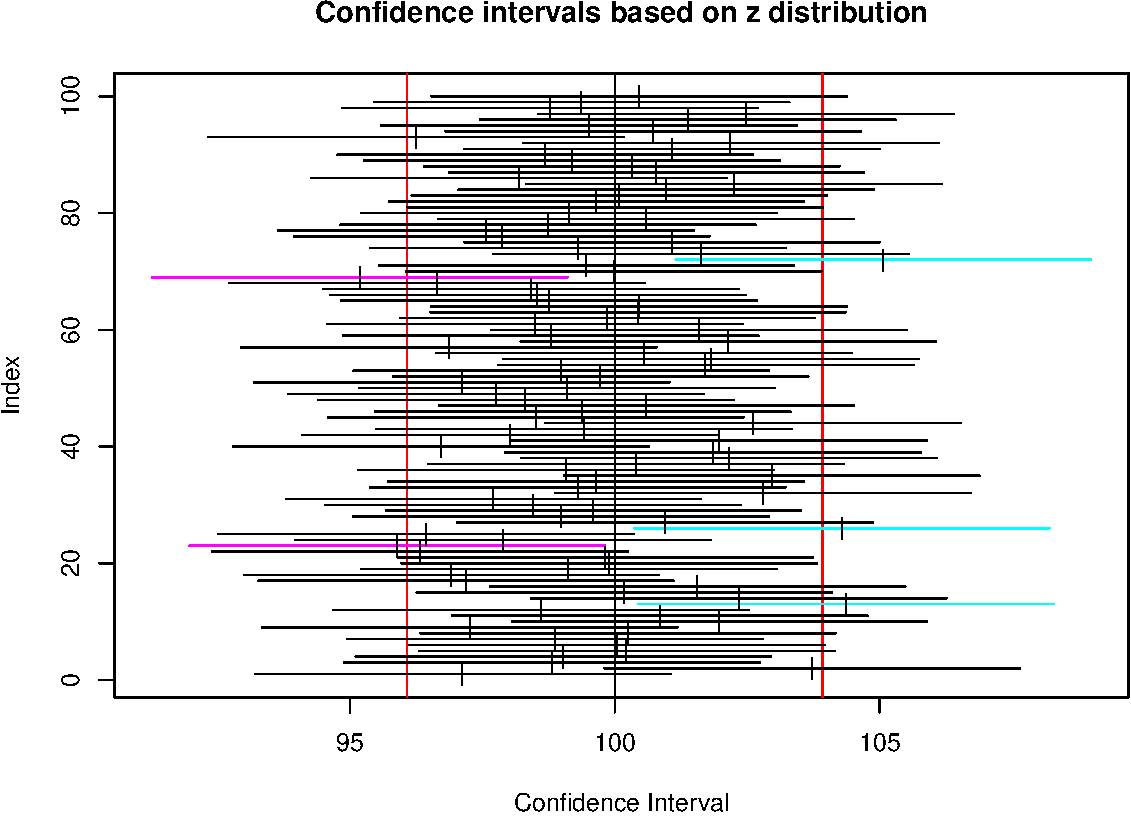
\includegraphics[width=1\textwidth]{figure/unnamed-chunk-1-1} 

}



\end{knitrout}
\end{frame}

\begin{frame}[fragile]{Intervalos de confiança para a média: $\sigma$ conhecido}
  \textbf{Exemplo}: Uma empresa de computadores deseja estimar o tempo médio de
  horas semanais que as pessoas utilizam o computador. Uma amostra
  aleatória de 25 pessoas apresentou um tempo médio
  de uso de 22,4 horas. Com base em estudos anteriores, a empresa assume
  que $\sigma = 5,2$ horas, e que os tempos são normalmente
  distribuídos.
  \begin{itemize}
  \item[a)] Verifique as suposições necessárias para o cálculo de
    um intervalo de confiança
  \item[b)] Para um nível de confiança de 95\%, encontre o valor crítico
    $z_{\alpha/2}$
  \item[c)] Calcule o erro máximo provável
  \item[d)] Construa o intervalo de confiança
  \item[e)] Escreva a interpretação do resultado
  \end{itemize}
\begin{knitrout}\footnotesize
\definecolor{shadecolor}{rgb}{0.969, 0.969, 0.969}\color{fgcolor}\begin{kframe}
\begin{verbatim}
Resp.: [20.362; 24.438]
\end{verbatim}
\end{kframe}
\end{knitrout}
\end{frame}

\begin{frame}{Intervalos de confiança para a média: $\sigma$ conhecido}
  %% magalhaes, cap. 7, pg 230--231
  A \textbf{amplitude} de um intervalo de confiança é dada pela
  diferença entre o  limite superior e inferior, ou seja,
  \begin{equation*}
    \text{AMP}_{IC} =
    \left[ \bar{x} + z_{\alpha/2} \cdot
      \left( \frac{\sigma}{\sqrt{n}} \right) \right] -
    \left[ \bar{x} - z_{\alpha/2} \cdot
      \left( \frac{\sigma}{\sqrt{n}} \right) \right]
    % = 2 \times z_{\alpha/2} \cdot (\sigma/\sqrt{n})
  \end{equation*}
  Note que, claramente, um intervalo de confiança depende conjuntamente
  de três componentes:
  \begin{itemize}
  \item nível de confiança $\gamma$, expresso pelo valor crítico
    $z_{\alpha/2}$
  \item desvio-padrão populacional $\sigma$
  \item tamanho da amostra $n$
  \end{itemize}
\end{frame}

\begin{frame}{Intervalos de confiança para a média: $\sigma$ conhecido}
  $z_{\alpha/2}$ Cada vez que aumentamos a confiança $\gamma$, o valor
  de $z_{\alpha/2}$ fica maior, e consequentemente a amplitude do
  intervalo aumenta.
  \begin{itemize}
  \item[] \small Intervalos maiores tem maior possibilidade de ``captura'' do
    verdadeiro valor de $\mu$
  \end{itemize}
  \vspace{1em}
  $\sigma$ Um grande desvio-padrão indica a possibilidade de um
  considerável distanciamento dos valores amostrais em relação à média
  populacional
  \begin{itemize}
  \item[] \small Ainda deve-se considerar que tanto $\bar{x}$ quanto
    $\sigma$ podem ser influenciados pela presença de valores extremos
  \end{itemize}
  \vspace{1em}
  $n$ Quanto maior for o tamanho da amostra, maior será a quantidade de
  informação disponível. Com isso, valores maiores de $n$ produzem
  intervalos mais informativos
  \begin{itemize}
  \item[] \small Para valores fixos de $\gamma$ e $\sigma$, valores
    maiores de $n$ produzem intervalos menores
  \end{itemize}
\end{frame}

\begin{frame}[fragile]{Intervalos de confiança para a média: $\sigma$ conhecido}
  % baseado em  magalhaes, cap 7, pg 238, ex. 18
  \textbf{Exemplo:} Seja $X \sim \N(\mu, 36)$
  \begin{itemize}
  \item[a)] Para uma amostra de tamanho 50, obtivemos média amostral
    18,5. Construa intervalos de confiança de
    \begin{itemize}
    \item[] (i) 90\% \quad (ii) 95\% \quad (iii) e 99\%
    \end{itemize}
  \item[b)] Calcule as amplitudes dos intervalos acima e explique a
    diferença.
  \item[c)] Para um nível de confiança de 95\%, construa intervalos de
    confiança (admita a mesma média amostral 18,5) supondo tamanhos de
    amostra
    \begin{itemize}
    \item[] (i) $n = 15$ \quad (ii) $n = 100$
    \end{itemize}
  \item[d)] Calcule as amplitudes dos intervalos acima e explique a
    diferença.
  \end{itemize}
\end{frame}

\begin{frame}[fragile]{Intervalos de confiança para a média: $\sigma$ conhecido}
Respostas do exercício anterior:
\begin{knitrout}\footnotesize
\definecolor{shadecolor}{rgb}{0.969, 0.969, 0.969}\color{fgcolor}\begin{kframe}
\begin{alltt}
\hlcom{## a)}
\end{alltt}
\begin{verbatim}
      (i)   (ii)  (iii)
LI 17.104 16.837 16.314
LS 19.896 20.163 20.686
\end{verbatim}
\begin{alltt}
\hlcom{## b)}
\end{alltt}
\begin{verbatim}
  (i)  (ii) (iii) 
2.792 3.326 4.372 
\end{verbatim}
\begin{alltt}
\hlcom{## c)}
\end{alltt}
\begin{verbatim}
      (i)   (ii)
LI 15.464 17.324
LS 21.536 19.676
\end{verbatim}
\begin{alltt}
\hlcom{## d)}
\end{alltt}
\begin{verbatim}
  (i)  (ii) 
6.072 2.352 
\end{verbatim}
\end{kframe}
\end{knitrout}

\end{frame}

\subsection{Determinação do tamanho amostral}

\begin{frame}{Determinação do tamanho amostral}
  Nosso objetivo é coletar dados para estimar a \textbf{média
    populacional} $\mu$ \\~\\
  A questão é:
  \begin{center}
    \textbf{Quantos elementos (itens, objetos, pessoas, \ldots) devemos
      amostrar?}
  \end{center}
  \vspace{1em}
  Já vimos que, de maneira (bem) geral, $n>30$ é um tamanho de amostra
  mínimo para a maioria dos casos. \\~\\
  Será que podemos ter uma estimativa melhor de quantos elementos
  devem ser amostrados para estimarmos a média populacional com uma
  precisão conhecida?
\end{frame}

\begin{frame}{Determinação do tamanho amostral}
  A partir da equação do \textbf{erro máximo provável}
  \begin{equation*}
    e = z_{\alpha/2} \cdot \frac{\sigma}{\sqrt{n}}
  \end{equation*}
  podemos isolar $n$ e chegar na seguinte equação para a determinação do
  tamanho amostral

  \begin{equation*}
    n = \left[ \frac{z_{\alpha/2} \cdot \sigma}{e} \right]^2
  \end{equation*}
\end{frame}

\begin{frame}{Determinação do tamanho amostral}
  Note que, em
  \begin{equation*}
    n = \left[ \frac{z_{\alpha/2} \cdot \sigma}{e} \right]^2
  \end{equation*}
  \begin{itemize}
  \item O tamanho amostral $n$ \textbf{não} depende do tamanho
    populacional $N$
  \item O tamanho amostral depende
    \begin{itemize}
    \item do nível de confiança desejado (expresso pelo valor crítico
      $z_{\alpha/2}$)
    \item do erro máximo \textsl{desejado}
    \item do desvio-padrão $\sigma$ (embora veremos que não é
      estritamente necessário)
    \end{itemize}
  \item Como o tamanho amostral precisa ser um número inteiro,
    arredondamos sempre o valor para o \textbf{maior} número inteiro
    mais próximo
  \end{itemize}
\end{frame}

\begin{frame}{Determinação do tamanho amostral}
  \textbf{Exemplo}: Seja $X \sim \text{N}(\mu,36)$
  \begin{itemize}
  \item[a)] Calcule o tamanho da amostra, para que com 95\% de
    probabilidade, a média amostral não difira da média populacional por
    mais de
    \begin{itemize}
    \item[] (i) 0,5 unidades \quad (ii) 2 unidades
    \end{itemize}
  \item[b)] Qual o impacto do erro máximo assumido para o tamanho da
    amostra?
  \item[c)] Calcule o tamanho da amostra, para que a diferença da média
    amostral para a média populacional (em valor absoluto) seja menor ou
    igual a 2 unidades, com níveis de confiança de
    \begin{itemize}
    \item[] (i) 90\% \quad (ii) 95\%
    \end{itemize}
  \item[d)] Compare as estimativas do item anterior e analise o impacto
    do nível de confiança para a determinação do tamanho amostral.
  \end{itemize}
\end{frame}

\begin{frame}[fragile]{Determinação do tamanho amostral}
Respostas do exercício anterior
\begin{knitrout}\footnotesize
\definecolor{shadecolor}{rgb}{0.969, 0.969, 0.969}\color{fgcolor}\begin{kframe}
\begin{alltt}
\hlcom{## a)}
\hlcom{# (i)}
\end{alltt}
\begin{verbatim}
[1] 554
\end{verbatim}
\begin{alltt}
\hlcom{# (ii)}
\end{alltt}
\begin{verbatim}
[1] 35
\end{verbatim}
\begin{alltt}
\hlcom{## c)}
\hlcom{# (i)}
\end{alltt}
\begin{verbatim}
[1] 25
\end{verbatim}
\begin{alltt}
\hlcom{# (ii)}
\end{alltt}
\begin{verbatim}
[1] 35
\end{verbatim}
\end{kframe}
\end{knitrout}
\end{frame}

\section{Intervalos de confiança para a média: $\sigma$ desconhecido}

\begin{frame}{Intervalos de confiança para a média: $\sigma$ desconhecido}
  Na maioria das situações práticas, não sabemos o verdadeiro valor do
  desvio-padrão populacional $\sigma$\\~\\
  Se não conhecemos $\sigma$, então não podemos usar a distribuição
  normal padrão ($Z$) para estimarmos a verdadeira média populacional
  $\mu$ \\~\\
  Nesse caso, usaremos a distribuição \textbf{$t$ de Student} que
  permite o uso da estimativa do \textbf{desvio-padrão amostral $s$} no
  lugar do valor desconhecido de $\sigma$.
\end{frame}

\begin{frame}{A distribuição $t$ de Student}
  Se uma população tem distribuição normal, então a distribuição da
  estatística

  \begin{equation*}
    t = \frac{\bar{x} - \mu}{s/\sqrt{n}} \, \sim \, t(n-1)
  \end{equation*}

  é uma \textbf{distribuição $t$ de Student} (ou simplesmente
  distribuição $t$) com $n-1$ \textbf{graus de liberdade}.\\~\\
\end{frame}

\begin{frame}{A distribuição $t$ de Student}
  Como não conhecemos $\sigma$, usamos o desvio-padrão amostral (não
  viesado):
  \begin{equation*}
    s = \sqrt{\frac{1}{n-1} \sum_{i=1}^{n} (x_i - \bar{x})^2}
  \end{equation*}
  mas isso introduz uma fonte de incerteza. \\~\\
  Para manter o nível de confiança desejado $\gamma$, compensamos essa
  incerteza calculando um intervalo de confiança um pouco maior: usando
  os valores críticos da distribuição $t_{\alpha/2;n-1}$ (ou
  simplesmente $t_{\alpha/2}$)
\end{frame}

\begin{frame}{A distribuição $t$ de Student}
  Para acharmos os valores críticos de $t_{\alpha/2;n-1}$, precisamos
  determinar o nível de confiança $\gamma = 1 - \alpha$ desejado e o
  valor dos \textbf{graus de liberdade} que indexa a distribuição $t$
  \begin{block}{Graus de liberdade (gl)}
    É o número de valores amostrais que podem variar depois que certas
    restrições tiverem sido impostas.
    \begin{equation*}
      gl = n-1
    \end{equation*}
  \end{block}
  Dada uma média, apenas $n-1$ valores podem ser associados
  \textbf{livremente}, antes que o último valor seja determinado.\\~\\
  %% portal action
  \textbf{Exemplo:} consideremos que 10 estudantes obtiveram média 8,0
  em um teste. Assim, a soma das 10 notas deve ser 80
  (restrição). Portanto, neste caso, temos $10-1=9$ graus de liberdade,
  pois as nove primeiras notas podem ser escolhidas aleatoriamente,
  contudo a 10$^{a}$ nota deve ser igual a [80 - (soma das 9 primeiras)].
  % Exemplo: A soma da nota máxima de 5 estudantes é 500. Se soubermos o
  % valor de notas de 4 deles, então a 5$^{a}$ nota estará
  % determinada. Como as 4 notas iniciais podem variar
  % \textbf{livremente}, dizemos que há 4 graus de liberdade
  % disponíveis.
\end{frame}

\begin{frame}{A distribuição $t$ de Student}
  Características da distribuição $t$
  \begin{itemize}
  \item É simétrica com média $t=0$ (assim como $z=0$)
  \item É diferente para tamanhos de amostra diferentes
  \item Possui maior área nas caudas e menor área no centro (quando
    comparada com a distribuição normal) $\rightarrow$ para incorporar a
    incerteza
  \item O desvio-padrão da distribuição $t$ varia com o tamanho da
    amostra (ao contrário da distribuição $z$ onde $\sigma=1$)
    \begin{itemize}
    \item $n$ $\downarrow$ \quad $\sigma$ $\uparrow$
    \item $n$ $\uparrow$ \quad $\sigma$ $\downarrow$
    \end{itemize}
  \item Á medida que o $n$ amostral aumenta, a distribuição $t$ se
    aproxima cada vez mais de uma distribuição normal padrão $Z$
    \begin{itemize}
    \item Por isso, para amostras grandes ($n>30$) o resultado das duas
      é similar
    \end{itemize}
  \end{itemize}
\end{frame}

\begin{frame}[fragile]{A distribuição $t$ de Student}
  %% \begin{figure}[p]
  %%   \centering
  %%   \includegraphics[width=.9\textwidth]{dist_t-crop}
  %% \end{figure}
\begin{knitrout}\footnotesize
\definecolor{shadecolor}{rgb}{0.969, 0.969, 0.969}\color{fgcolor}

{\centering 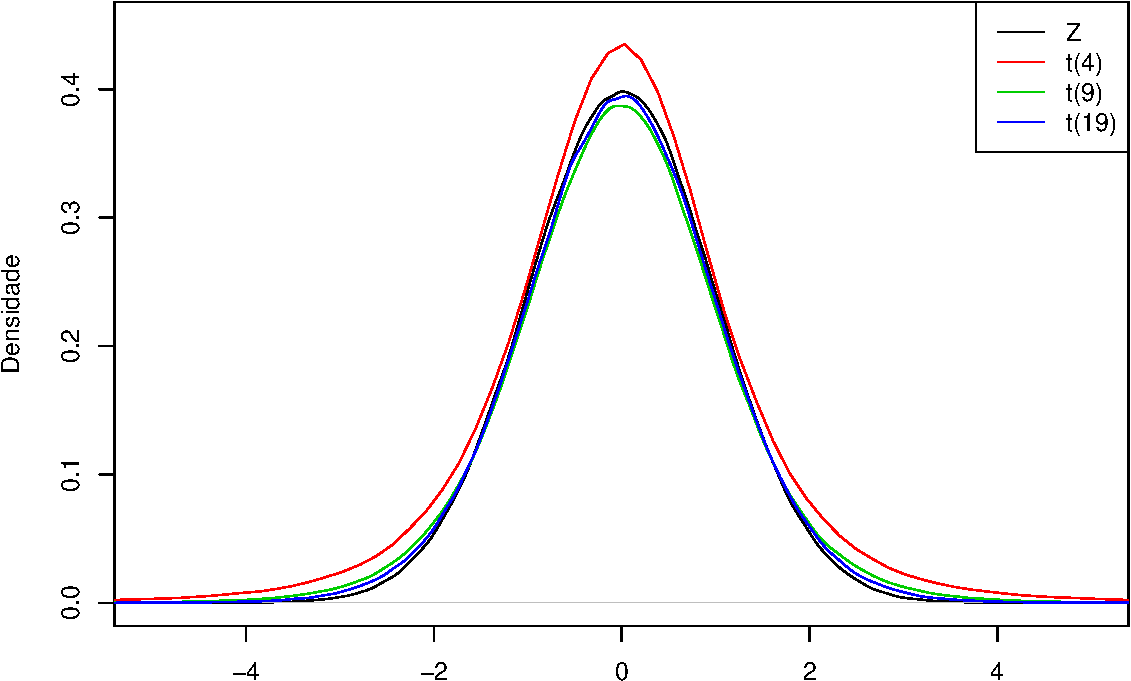
\includegraphics[width=1\textwidth]{figure/unnamed-chunk-5-1} 

}



\end{knitrout}
\end{frame}

\begin{frame}{Encontrando valores críticos de $t$}
  Com a definição do \textbf{nível de confiança} e sabendo o tamanho da
  amostra $n$, sabemos então o valor de $\alpha$ e dos gl, e devemos
  encontrar o valor de $t_{\alpha/2;n-1}$. Usando
  como exemplo $\gamma = 0,95 = 1 - 0,05 \Rightarrow \alpha = 0,05$ ou
  5\% e uma amostra de $n=7$
  \vspace{1em}
  \begin{itemize}
  \item Temos que $n=7 \Rightarrow gl = n-1 = 6$
  \item Na tabela da distribuição $t$ de Student procure a linha
    correspondente aos gl, e à coluna correspondente ao valor de
    $\alpha$
  \item O valor de $t_{\alpha/2;n-1}$ será determinado pelos valores
    correspondentes \textbf{no corpo da tabela}. Nesse caso,
    $t_{\alpha/2;n-1} = 2,447$ é o valor crítico procurado.
  \end{itemize}
\end{frame}

\begin{frame}{Encontrando valores críticos de $t$}
  %% Ex 6.10, pg 202 do Spiegel
  Sabemos que o valor crítico de 95\% de confiança para a distribuição
  normal padrão é $z_{\alpha/2} = 1,96$. Quais são os valores críticos
  correspondentes para a distribuição $t$, se o $n$ amostral for
  \begin{itemize}
  \item $n=10$
  \item $n=21$
  \item $n=30$
  \item $n=61$
  \item $n=100$
  \item $n=1000$
  \end{itemize}
  Verifique também os 4 primeiros valores para $\gamma = 0,9$ e $\gamma
  = 0,99$
  % \begin{table}[h]
  %   \centering
  %   \begin{tabular}{ccc}
  %     \hline
  %     Nível de confiança $\gamma$ & $\alpha$ & Valor crítico
  %     $z_{\alpha/2}$ \\
  %     \hline
  %     0,90 & 0,10 & 1,645 \\
  %     0,95 & 0,05 & 1,96 \\
  %     0,99 & 0,01 & 2,575 \\
  %     \hline
  %   \end{tabular}
  % \end{table}
\end{frame}

\begin{frame}{Intervalos de confiança para a média: $\sigma$ desconhecido}
  Com estas definições, podemos construir um intervalo de confiança para
  uma estimativa da média amostral com $\sigma$ desconhecido através de
  \begin{equation*}
    \bar{x} - e < \mu < \bar{x} + e
  \end{equation*}
  com
  \begin{equation*}
    e = t_{\alpha/2} \cdot \left(\frac{s}{\sqrt{n}}\right)
  \end{equation*}
  Outras notações
  \begin{equation*}
    \bar{x} \pm e
  \end{equation*}
  \begin{equation*}
    [\bar{x} - e; \bar{x} + e]
  \end{equation*}
\end{frame}

\begin{frame}{Intervalos de confiança para a média: $\sigma$ desconhecido}
  \textbf{Procedimentos gerais para a construção de intervalos de
    confiança com $\sigma$ desconhecido}
  \\~\\
  \begin{enumerate}
  \item Verifique se as suposições necessárias estão satisfeitas
    \begin{itemize}
    \item Temos uma AAS
    \item Temos uma estimativa de $s$
    \item \textsl{A população tem distribuição normal ou $n>30$}
      $\leftarrow$ este requisito não é mandatório, pois a distribuição
      $t$ irá se ``ajustar'' para acomodar a incerteza de amostras
      pequenas
    \end{itemize}
  \item Determine o nível de confiança $\gamma$, e identifique $\alpha$
  \item Com o valor de $\alpha$ definido, e o valor dos \textbf{graus de
    liberdade} $gl=n-1$, encontre o valor crítico de $t_{\alpha/2;n-1}$
  \item Calcule a margem de erro $e = t_{\alpha/2} \cdot (s/\sqrt{n})$
  \item Coloque em um dos formatos gerais para intervalo de confiança
    \begin{itemize}
    \item[] $\bar{x} - e < \mu < \bar{x} + e$
    \item[] $\bar{x} \pm e$
    \item[] $[\bar{x} - e; \bar{x} + e]$
    \end{itemize}
  \end{enumerate}
\end{frame}

\begin{frame}{Intervalos de confiança para a média: $\sigma$ desconhecido}
  %% Triola pg 291
  Exemplo: Em um teste da eficácia do alho na dieta para a redução do
  colesterol, 49 pessoas foram avaliadas e seus níveis de colesterol
  foram medidos antes e depois do tratamento. As \textbf{mudanças} nos
  níveis de colesterol apresentaram média de 0,4 e desvio-padrão de
  21.

  \begin{itemize}
  \item[a)] Verifique as suposições necessárias para o cálculo do intervalo
    de confiança
  \item[b)] Para um nível de confiança de 95\%, encontre o valor crítico
    $t_{\alpha/2;n-1}$
  \item[c)] Calcule o erro máximo provável
  \item[d)] Construa o intervalo de confiança
  \item[e)] Escreva a interpretação do resultado
  \item[f)] O que o intervalo de confiança sugere sobre a eficácia do uso do
    alho na dieta para a redução do colesterol?
  \end{itemize}
  Resolva o mesmo exemplo supondo que o $\sigma = s$ é conhecido (ou
  seja, usando a distribuição $Z$). Compare os dois métodos.
\end{frame}

\begin{frame}[fragile]{Intervalos de confiança para a média: $\sigma$ desconhecido}
Respostas do exercício anterior:
\begin{itemize}
\item Usando a distribuição $t$
\begin{knitrout}\footnotesize
\definecolor{shadecolor}{rgb}{0.969, 0.969, 0.969}\color{fgcolor}\begin{kframe}
\begin{verbatim}
$`valor critico`
[1] 2.0086

$`margem de erro`
[1] 5.9063

$`intervalo de confiança`
[1] -5.5063  6.3063
\end{verbatim}
\end{kframe}
\end{knitrout}
\item Usando a distribuição $z$
\begin{knitrout}\footnotesize
\definecolor{shadecolor}{rgb}{0.969, 0.969, 0.969}\color{fgcolor}\begin{kframe}
\begin{verbatim}
$`valor critico`
[1] 1.96

$`margem de erro`
[1] 5.8799

$`intervalo de confiança`
[1] -5.4799  6.2799
\end{verbatim}
\end{kframe}
\end{knitrout}
\end{itemize}
\end{frame}

\begin{frame}{Diferenças entre $z$ e $t$}
  Para o mesmo exemplo anterior, assuma que foram avaliadas apenas 8
  pessoas. Calcule intervalos de confiança para a média, $\bar{x} = 0,4$
  usando
  \begin{itemize}
  \item a distribuição $t$ (ou seja, assumindo $\sigma$ desconhecido,
  portanto $s = 21$)
\item a distribuição $Z$ (ou seja, assumindo $\sigma$ conhecido,
  portanto $\sigma = 21$)
  \end{itemize}
  Qual a sua conclusão referente à diferença observada entre os dois
  intervalos de confiança? Por que ocorre essa diferença?
\end{frame}

\begin{frame}[fragile]{Intervalos de confiança para a média: $\sigma$ desconhecido}
Respostas do exercício anterior:
\begin{itemize}
\item Usando a distribuição $t$
\begin{knitrout}\footnotesize
\definecolor{shadecolor}{rgb}{0.969, 0.969, 0.969}\color{fgcolor}\begin{kframe}
\begin{verbatim}
$`valor critico`
[1] 2.3646

$`margem de erro`
[1] 17.556

$`intervalo de confiança`
[1] -17.156  17.956
\end{verbatim}
\end{kframe}
\end{knitrout}
\item Usando a distribuição $z$
\begin{knitrout}\footnotesize
\definecolor{shadecolor}{rgb}{0.969, 0.969, 0.969}\color{fgcolor}\begin{kframe}
\begin{verbatim}
$`valor critico`
[1] 1.96

$`margem de erro`
[1] 14.552

$`intervalo de confiança`
[1] -14.152  14.952
\end{verbatim}
\end{kframe}
\end{knitrout}
\end{itemize}
\end{frame}

\begin{frame}{Escolha entre $z$ e $t$}
  \begin{table}[h]
    \centering
    \begin{tabular}{lp{6cm}}
      \hline
      \textbf{Método} & \textbf{Condições} \\
      \hline
      Distribuição normal ($Z$) & $\sigma$ conhecido e população
      normalmente distribuída \\
                                & ou \\
                                & $\sigma$ conhecido e $n>30$ \\
     \hline
     Distribuição $t$ & $\sigma$ desconhecido e população normalmente
     distribuída \\
                     & ou \\
                     & $\sigma$ desconhecido e $n>30$ \\
    \hline
    \end{tabular}
  \end{table}
\end{frame}

\begin{frame}{Escolha entre $z$ e $t$}
  Nos exemplos abaixo, indique se é mais apropriado usar o valor crítico
  de $z_{\alpha/2}$ (da distribuição normal), de $t_{\alpha/2}$ (da
  distribuição $t$), ou nenhum deles
  \begin{itemize}
  \item[a)] $n=9,\, \bar{x}=75,\, s=15$, população com distribuição
    normal
  \item[b)] $n=5,\, \bar{x}=20,\, s=2$, população com distribuição
    muito assimétrica
  \item[c)] $n=12,\, \bar{x}=98,6,\, \sigma=0,6$, população com
    distribuição normal
  \item[d)] $n=75,\, \bar{x}=98,6,\, \sigma=0,6$, população com
    distribuição assimétrica
  \item[e)] $n=75,\, \bar{x}=98,6,\, s=0,6$, população com
    distribuição assimétrica
  \end{itemize}
\end{frame}

\subsection{Determinação do tamanho amostral}

\begin{frame}{Determinação do tamanho amostral}
  Se $\sigma$ for desconhecido?\\~\\
  \begin{enumerate}
  \item Estime o valor de $\sigma$ com base em algum estudo feito
    anteriormente
  \item Faça uma amostra piloto e estime o desvio-padrão amostra $s$, e
    use-o como uma aproximação para o desvio-padrão populacional $\sigma$
  \item Use a \textbf{regra empírica} da amplitude para dados com
    distribuição (aproximadamente) normal
  \end{enumerate}
\end{frame}

\begin{frame}{Determinação do tamanho amostral}
  Regra empírica para uma distribuição (aproximadamente) normal
  \begin{figure}[h]
    \centering
    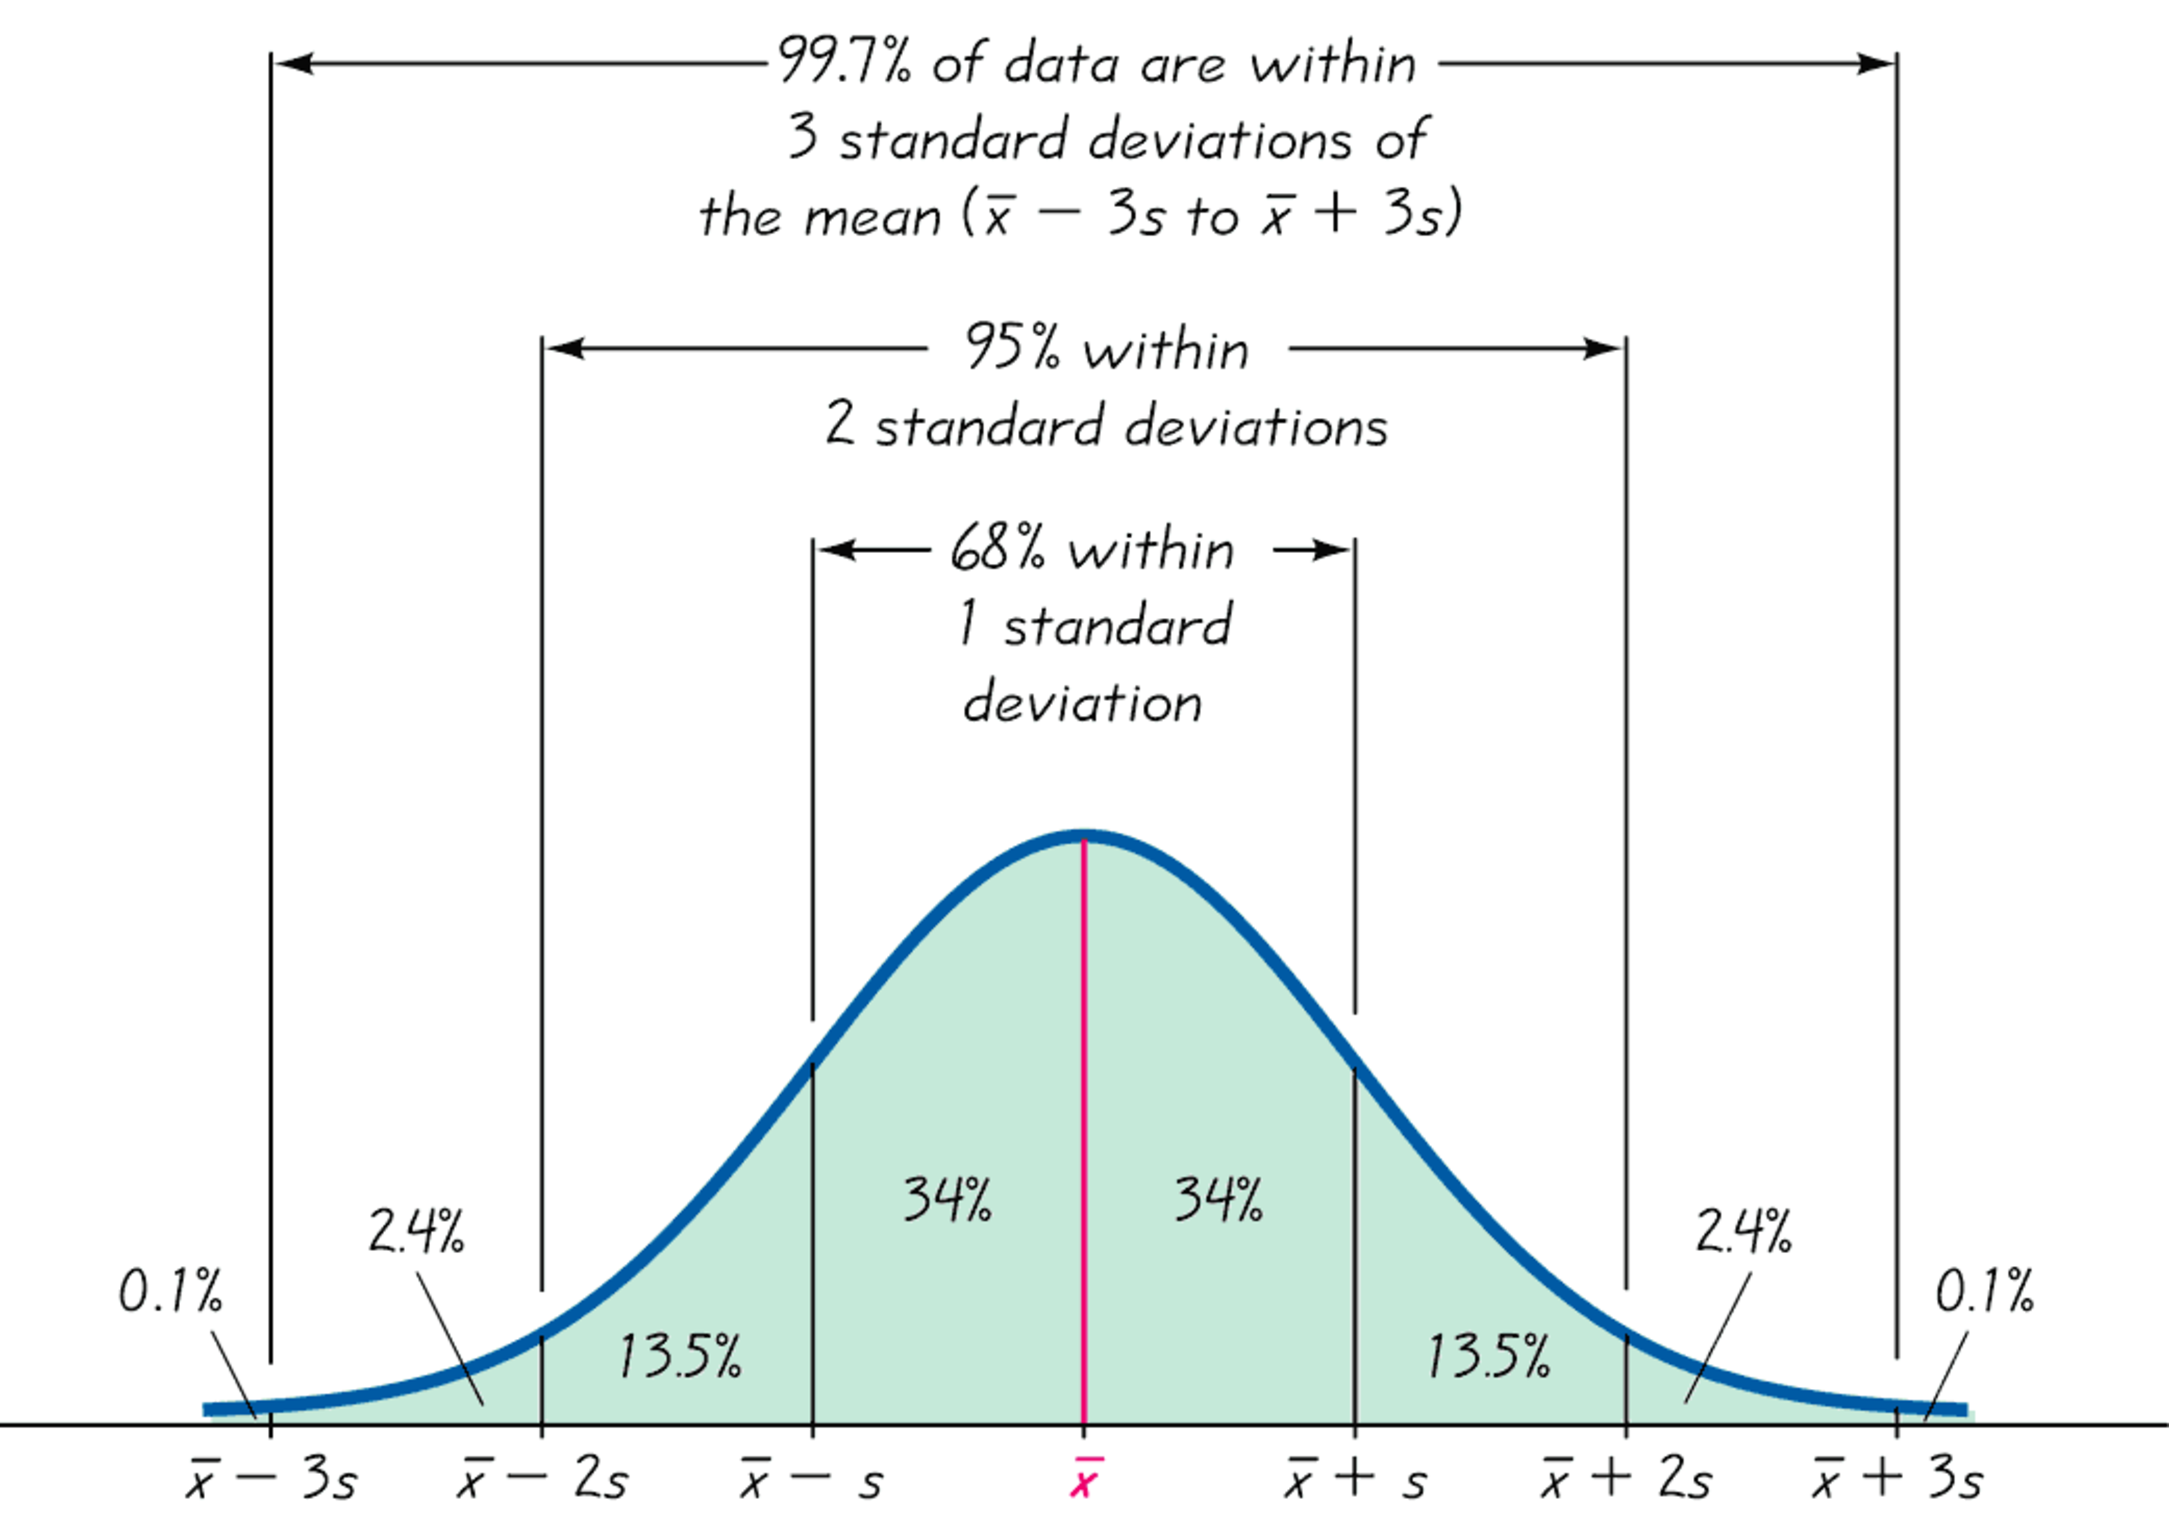
\includegraphics[width=.8\textwidth]{empirica}
  \end{figure}
\end{frame}

\begin{frame}{Determinação do tamanho amostral}
  Regra empírica para uma distribuição (aproximadamente) normal\\~\\
  Define-se \textbf{valores usuais} aqueles que são típicos e não muito
  extremos. \\~\\
  Como sabemos que em uma distribuição (aproximadamente) normal, 95\%
  dos dados encontram-se a 2 desvios-padrões acima e abaixo da média,
  temos que
  \begin{eqnarray*}
    4\sigma &=& (\max - \min) \\
    \sigma &=& \frac{(\max - \min)}{4}
  \end{eqnarray*}
\end{frame}

\begin{frame}[fragile]{Determinação do tamanho amostral}
  Exemplo: Um professor deseja estimar o salário médio de professores
  do ensino médio de uma cidade. Quantos professores devem ser
  selecionados para termos 90\% de confiança que a média amostral esteja
  a menos de R\$30,00 da média populacional? Sabe-se apenas que os
  salários variam entre R\$800,00 e R\$1.200,00.\\~\\
  Use
  \begin{equation*}
    n = \left[ \frac{z_{\alpha/2} \cdot \sigma}{e} \right]^2
  \end{equation*}
\begin{knitrout}\footnotesize
\definecolor{shadecolor}{rgb}{0.969, 0.969, 0.969}\color{fgcolor}\begin{kframe}
\begin{alltt}
\hlcom{## Estimativa de sigma pela regra empírica}
\end{alltt}
\begin{verbatim}
[1] 100
\end{verbatim}
\begin{alltt}
\hlcom{## Tamanho da amostra}
\end{alltt}
\begin{verbatim}
[1] 31
\end{verbatim}
\end{kframe}
\end{knitrout}
\end{frame}

\section{Intervalo de confiança para a proporção $p$}

\begin{frame}{Intervalo de confiança para a proporção $p$}
  Em muitas situações, estamos interessados em estudar uma
  \textbf{proporção}, ao invés da média \\~\\
  Por exemplo:
  \begin{itemize}
  \item a proporção de eleitores de um determinado candidato
  \item a proporção de peças defeituosas em um processo industrial
  \item a proporção de alunos reprovados na disciplina de estatística
  \end{itemize}
  \vspace{1em}
  Nestes casos, a \textbf{distribuição binomial} deve ser utilizada no
  processo de inferência.
\end{frame}

\begin{frame}{Intervalo de confiança para a proporção $p$}
  A proporção amostral
  \begin{equation*}
    \hat{p} = \frac{x}{n} = \frac{\text{número de sucessos}}{\text{total de
        tentativas}}
  \end{equation*}
  é a ``melhor estimativa'' para a proporção populacional $p$ \\~\\
  Exemplo: em 5 lançamentos de uma moeda considere que o evento ``cara''
  (Ca) seja o sucesso (``sucesso'' = 1; ``fracasso'' = 0). Um possível
  resultado seria o conjunto $\{Ca, Ca, Co, Co, Ca\}$. A proporção
  amostral seria
  \begin{equation*}
    \hat{p} = \frac{\text{número de sucessos}}{\text{total de
        tentativas}} = \frac{3}{5} = 0,6
  \end{equation*}
  % \begin{table}[h]
  %   \centering
  %   \begin{tabular}{ll}
  %     Realização & $X$ \\
  %     Ca & 1 \\
  %     Ca & 1 \\
  %     Co & 0 \\
  %     Co & 0 \\
  %     Ca & 1 \\
  %   \end{tabular}
  % \end{table}
\end{frame}

\begin{frame}{Distribuição amostral de uma proporção}
Através do estudo da distribuição amostral da proporção, chegamos aos
seguintes resultados
\begin{itemize}
\item $\E(\hat{p}) = \mu_{\hat{p}} = p$
\item $\Var(\hat{p}) = \sigma^{2}_{\hat{p}} = \frac{p(1-p)}{n}$
\end{itemize}
Ou seja,
\begin{equation*}
  p \sim \N \left( p, \frac{p(1-p)}{n} \right)
\end{equation*}
Ainda podemos mostrar que a quantidade
\begin{equation*}
  Z = \frac{\hat{p} - p}{\sqrt{\frac{p(1-p)}{n}}} \, \sim \, \N(0,1)
\end{equation*}
Quando não conhecemos $p$, usamos $\hat{p}=x/n$ como estimativa
%% \begin{enumerate}
%% \item A proporção amostral $p$ \textbf{tende} para o valor da proporção
%%   populacional $\pi$
%% \item A distribuição das proporções amostrais tende a ser uma
%%   \textbf{distribuição normal}
%% \end{enumerate}
\end{frame}

\begin{frame}{Intervalo de confiança para a proporção $p$}
  Com estas definições, podemos construir um intervalo de confiança para
  uma estimativa da proporção amostral $p$ através de
  \begin{equation*}
    \hat{p} - e < p < \hat{p} + e
  \end{equation*}
  com
  \begin{equation*}
    e = z_{\alpha/2} \cdot \sqrt{\frac{p(1-p)}{n}}
  \end{equation*}
  Outras notações
  \begin{equation*}
    \hat{p} \pm e
  \end{equation*}
  \begin{equation*}
    [\hat{p} - e; \hat{p} + e]
  \end{equation*}
\end{frame}

\begin{frame}{Intervalo de confiança para a proporção $p$}
  \textbf{Procedimentos gerais para a construção de intervalos de
    confiança para a proporção $p$}
  \\~\\
  \begin{enumerate}
  \item Verifique se as suposições necessárias estão satisfeitas
    \begin{itemize}
    \item Temos uma AAS
    \item As condições para a distribuição binomial são satisfeitas
      \begin{itemize}
      \item as tentativas são independentes
      \item há duas categorias de resultado (``sucesso'', ``fracasso'')
      \item a probabilidade de sucesso $p$ permanece constante
      \end{itemize}
    \item A distribuição normal pode ser usada como aproximação para a
      distribuição binomial, ou seja, $np \geq 5$ e $n(1-p) \geq 5$
    \end{itemize}
  \item Determine o nível de confiança $\gamma$, e identifique $\alpha$
  \item Com o valor de $\alpha$ definido, encontre o valor crítico de
    $z_{\alpha/2}$
  \item Calcule a margem de erro $e = z_{\alpha/2} \cdot
    \sqrt{\frac{p(1-p)}{n}}$
  \item Coloque em um dos formatos gerais para intervalo de confiança
    \begin{itemize}
    \item[] $\hat{p} - e < \pi < \hat{p} + e$
    \item[] $\hat{p} \pm e$
    \item[] $[\hat{p} - e; \hat{p} + e]$
    \end{itemize}
  \end{enumerate}
\end{frame}

\begin{frame}{Intervalo de confiança para a proporção $p$}
  Exemplo: em uma pesquisa realizada por um instituto de pesquisa
  Norte-Americano, 1500 adultos foram selecionados aleatoriamente para
  responder à pergunta se acreditam ou não no aquecimento global. 1050
  entrevistados respoderam que sim. Com isso:
  \begin{itemize}
  \item[a)] Verifique as suposições para o cálculo do intervalo de confiança
  \item[b)] Para um nível de confiança de 95\%, encontre o valor crítico
    de $z_{\alpha/2}$
  \item[c)] Calcule o erro máximo provável
  \item[d)] Construa o intervalo de confiança para $p$
  \item[e)] Escreva a interpretação do resultado
  \item[f)] Com base nesse resultado, podemos concluir que a maioria dos
    adultos acredita no aquecimento global?
  \end{itemize}
\end{frame}

\begin{frame}[fragile]{Intervalo de confiança para a proporção $p$}
Resposta do exercício anterior:
\begin{knitrout}\footnotesize
\definecolor{shadecolor}{rgb}{0.969, 0.969, 0.969}\color{fgcolor}\begin{kframe}
\begin{verbatim}
$`valor critico`
[1] 1.96

$`margem de erro`
[1] 0.023191

$`intervalo de confiança`
[1] 0.67681 0.72319
\end{verbatim}
\end{kframe}
\end{knitrout}
\end{frame}

\subsection{Determinação do tamanho amostral}

\begin{frame}{Determinação do tamanho amostral}
  A partir da equação do erro máximo provável
  \begin{equation*}
    e = z_{\alpha/2} \cdot \sqrt{\frac{p(1-p)}{n}}
  \end{equation*}
  podemos isolar $n$ e chegar na seguinte equação para a determinação do
  tamanho amostral para uma proporção populacional

  \begin{equation*}
    n = \left( \frac{z_{\alpha/2}}{e} \right)^2 \cdot p(1-p)
  \end{equation*}
\end{frame}

\begin{frame}{Determinação do tamanho amostral}
  Quando conhecemos a verdadeira proporção populacional $p$, podemos
  usá-la para calcular o $n$ a partir da expressão acima. \\~\\
  Quando \textbf{não conhecemos} a proporção poppulacional $p$, usamos
  como estimativa $p=0,5$ porque
  \begin{table}[h]
    \centering
    \begin{tabular}{ccc}
      \hline
      $p$ & $(1-p)$ & $p(1-p)$ \\
      \hline
      0,1 & 0,9 & 0,09 \\
      0,3 & 0,7 & 0,21 \\
      0,5 & 0,5 & \textbf{0,25} \\
      0,6 & 0,4 & 0,24 \\
      0,8 & 0,2 & 0,16 \\
      \hline
    \end{tabular}
  \end{table}
  Quando $p=0,5$ teremos o maior tamanho de amostra possível.
\end{frame}

\begin{frame}[fragile]{Determinação do tamanho amostral}
  Exemplo: um fabricante de peças deseja estimar a verdadeira
  proporção de peças defeituosas no processo de fabricação, com um erro
  máximo de 3\% e nível de confiança de 99\%. Calcule o tamanho da
  amostra necessário para se estimar esta proporção se:
  \begin{itemize}
  \item[a)] O fabricante acredita que aproximadamente 10\% de seus produtos
    são defeituosos.
  \item[b)] O fabricante não tem nenhuma informação prévia sobre a proporção
    de peças defeituosas.
  \end{itemize}
\begin{knitrout}\footnotesize
\definecolor{shadecolor}{rgb}{0.969, 0.969, 0.969}\color{fgcolor}\begin{kframe}
\begin{alltt}
\hlcom{## a)}
\end{alltt}
\begin{verbatim}
[1] 664
\end{verbatim}
\begin{alltt}
\hlcom{## b)}
\end{alltt}
\begin{verbatim}
[1] 1844
\end{verbatim}
\end{kframe}
\end{knitrout}
\end{frame}

\section{Referências}

\begin{frame}{Referências}
  \begin{itemize}
  \item Bussab, WO; Morettin, PA. \textbf{Estatística básica}. São
    Paulo: Saraiva, 2006. [Cap. 11]
  \item Magalhães, MN; Lima, ACP. \textbf{Noções de Probabilidade e
      Estatística}. São Paulo: EDUSP, 2008. [Cap. 7]
  \item Montgomery, DC; Runger, GC. \textbf{Estatística aplicada e
      probabilidade para engenheiros}. Rio de Janeiro: LTC Editora,
    2012. [Cap. 8]
  \end{itemize}
\end{frame}

\end{document}
